\documentclass{beamer}
\usepackage[utf8]{inputenc}
\usepackage{listings}
\usepackage{booktabs}
\usepackage{amssymb}
\usepackage{amsmath}
\usepackage{nicefrac}
\usepackage{bm}
\usepackage{enumitem}
\usepackage{hyperref}
\usepackage[export]{adjustbox}
\usepackage{svg}

\usetheme{Madrid}
\definecolor{mlpblue}{rgb}{0.1, 0.14, 0.24}

\useoutertheme{infolines} % Alternatively: miniframes, infolines, split
\useinnertheme{circles}
\usecolortheme[named=mlpblue]{structure}

\lstset{basicstyle=\footnotesize\ttfamily,breaklines=true}

%------------------------------------------------------------
%This block of code defines the information to appear in the
%Title page
\title[Transformers]{Attention Is All You Need:}

\subtitle{Deriving the Seminal Transformer Architecture from First Principles}

\author[Machine Learning @ Purdue] % optional
{J.~Setpal} 

\date{September 3, 2024}

\titlegraphic{
\includegraphics[width=7cm]{../shared/logo-long.pdf}}

%End of title page configuration block
%------------------------------------------------------------

%The next block of commands puts the table of contents at the 
%beginning of each section and highlights the current section:

% \AtBeginSection[]
% {
%   \begin{frame}
%     \frametitle{Outline}
%     \tableofcontents[currentsection]
%   \end{frame}
% }
% ------------------------------------------------------------


\begin{document}

\frame{\titlepage}


%---------------------------------------------------------
% This block of code is for the table of contents after
% the title page
% \begin{frame}
% \frametitle{Outline}
% \tableofcontents
% \end{frame}
%---------------------------------------------------------

\begin{frame}{Glossary}
	Some context-relevant terms:
	\begin{enumerate}[label=\alph*.]
		\item \textbf{Neuron:} The unit of a nueral network $y = \sigma(XW)$
		\item \textbf{Logit:} Pre-activation scores for the \textit{final layer}.
		\item \textbf{Dot / Inner Product:} $\langle a, b \rangle = \sum^N_{i=1}a_ib_i$
		\item \textbf{Matrix Multiplication:} For $X \in \mathbb{R}^{a \times b},\ Y \in \mathbb{R}^{b \times c}$, $Z = XY \in \mathbb{R}^{a \times c}\ s.t.\ z_{ij} = \sum^b_{k=1} a_{ik} b_{kj}$
		\item \textbf{Activation:} Non-linear function over the output of matrix multiplication.
		\item \textbf{Gradient:} $\nabla_w \mathcal{L}(w)$, derivative of $\mathcal{L}: \mathbb{R}^a \rightarrow \mathbb{R}$
		\item \textbf{Latent Vector:} $h^{(\ell)}$, intermediary output from within a neural network.
		\item \textbf{Embedding:} A look-up table that translates categorical values (words) to vectors.
	\end{enumerate}
\end{frame}

\begin{frame}{Some Intuitive Insights}
	\textbf{Q:} Differentiate between the meanings of each underlined word below:
	\begin{enumerate}[label=\alph*.]
		\item I had a picnic by the river \underline{bank} yesterday.
		\item I am NOT going to rob a \underline{bank} tomorrow at 8:30am ET.
	\end{enumerate} \pause

	\textbf{Insight:} Context is important. \pause \newline \\

	$n$-gram models use the following (Markov) assumption:
	\begin{gather}
	p\left(x_t | \{x_i\}^{t-1}_{i=1};\theta\right) \approx p\left(x_t | x_{t-1};\theta\right)
	\end{gather} \pause \vspace{-1.5em}
	This is \textbf{incorrect.} \pause Context is important!
\end{frame}

\begin{frame}{How Expensive is Context?}
	\textbf{Q:} So, why do $n$-gram models use the Markov assumption? \pause \\
	\textbf{A:} Efficiency. \pause \newline \\

	\textbf{Q:} Can we do better? \pause \\
	\textbf{A:} Yes. Enter, Recurrent Neural Networks (RNNs):

	\begin{columns}
		\begin{column}{.5\textwidth}
			\begin{center}
				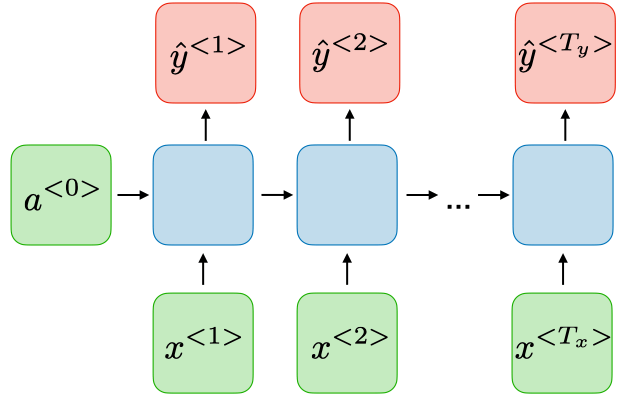
\includegraphics[width=\textwidth]{img/rnn.png} 
			\end{center} \pause
		\end{column}
		\begin{column}{.5\textwidth}
			Here, a hidden representation $a^{\langle \ell \rangle}$ is propogated, encoding relevant context. \pause \newline \\
			\textbf{Caveat:} $a^{\langle \ell \rangle} \in \mathbb{R}^d$, with \textit{fixed} $d$. \pause \\
			This mitigates capability for long-term memory \& recollection.
		\end{column}
	\end{columns}
\end{frame}

\begin{frame}{Now, Let's Pay Attention}
	One way to improve this is by incorporating \textit{attention} into RNNs.\footnote{\tiny \url{https://distill.pub/2016/augmented-rnns/\#attentional-interfaces}} \pause \newline \\

	\textbf{Q:} Well, what does it mean to ``incorporate attention''? \pause \\
	\textbf{A:} For latent vectors $\{\ell_i\}^N_{i=1}$:
	\begin{gather}
		a^{\langle \ell \rangle} = \sum^{N}_{i=1} w_i^{(\ell)} \ell_i \quad \text{where} \quad \sum^N_{i=1}w_i^{(\ell)} = 1,\ w_i^{(\ell)} \geq 0 ~\forall i, \ell
	\end{gather} \pause

	\begin{center}
		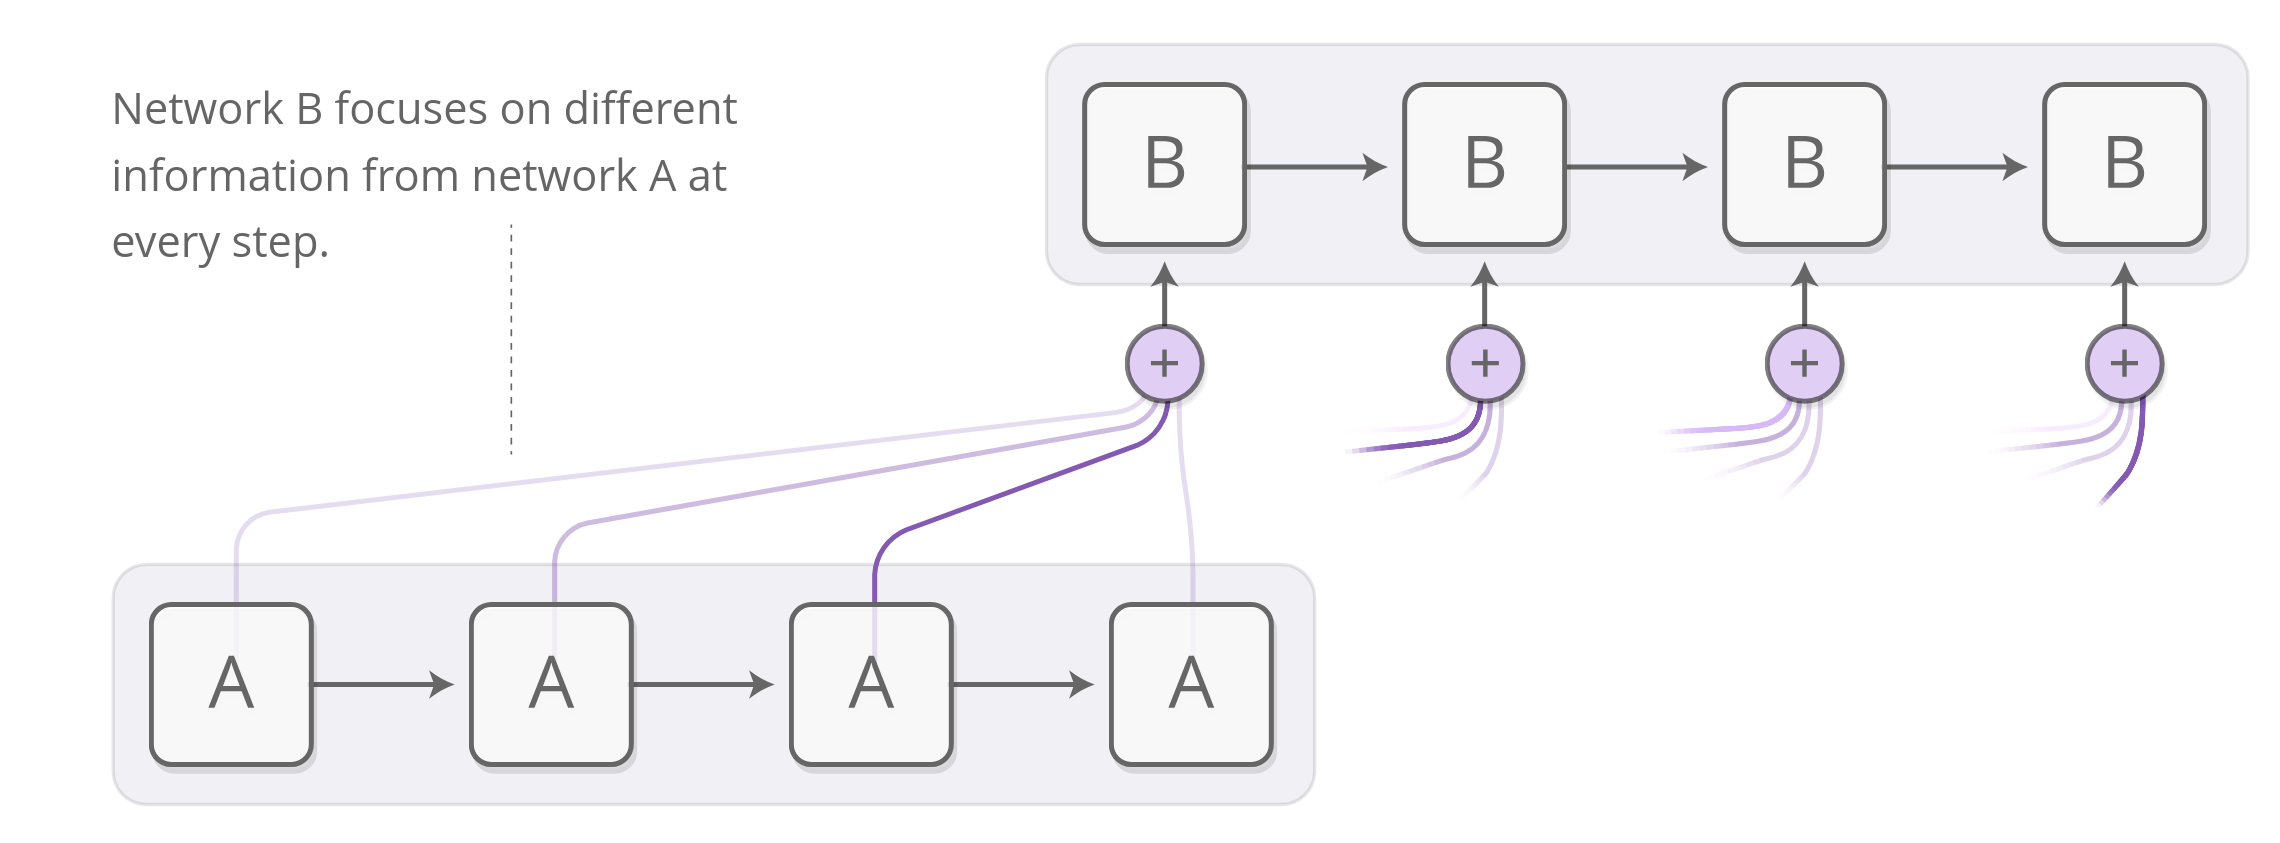
\includegraphics[width=.8\textwidth]{img/rnn-attention.png}
	\end{center}
\end{frame}

\begin{frame}{Self-Attention ($\nicefrac{1}{2}$)}
	Self-Attention makes attention self-referential, by effectively creating a \textbf{trainable database}. \pause \newline \\

	We query this database to extract important information from our input sequence. For $\{x_i\}^t_{i=1}$,
	\begin{gather}
		W_Q, W_K, W_V \in \mathbb{R}^{d_{in} \times d_{out}} \\
		K = X W_K, 
		Q = X W_Q, 
		V = X W_V \\
		\uncover<+(1)->{\alpha_i = \sigma_{softmax}\left(\frac{q_i k_i^T}{\sqrt{d_k}}\right)} \\
		\uncover<+(1)->{h(x) = \sum^t_{i=1} \alpha_i v_i}
	\end{gather} \pause
	Where $q_i, k_i, v_i$ are each independently computed latent matrices.
	\begin{gather}
		\text{Self-Attention}(Q, K, V) = \left(\frac{QK^T}{\sqrt{d_{out}}}\right) V
	\end{gather}
\end{frame}

\begin{frame}{Positional Encoding}
	A consequence of this setup, howeveer is that we are not considering the order of the tokens anymore. It is \textbf{permutation invariant}. \pause \newline \\

	To resolve this, we add positional encodings to each word embedding:
	\vspace{-.75em}
	\begin{gather}
		PE_{(pos, 2i)} = \sin(\nicefrac{pos}{1E4^{\nicefrac{2i}{d_{model}}}}) \\
		PE_{(pos, 2i+1)} = \cos(\nicefrac{pos}{1E4^{\nicefrac{2i}{d_{model}}}})
	\end{gather}
	\begin{center}
		\vspace{-.75em}
		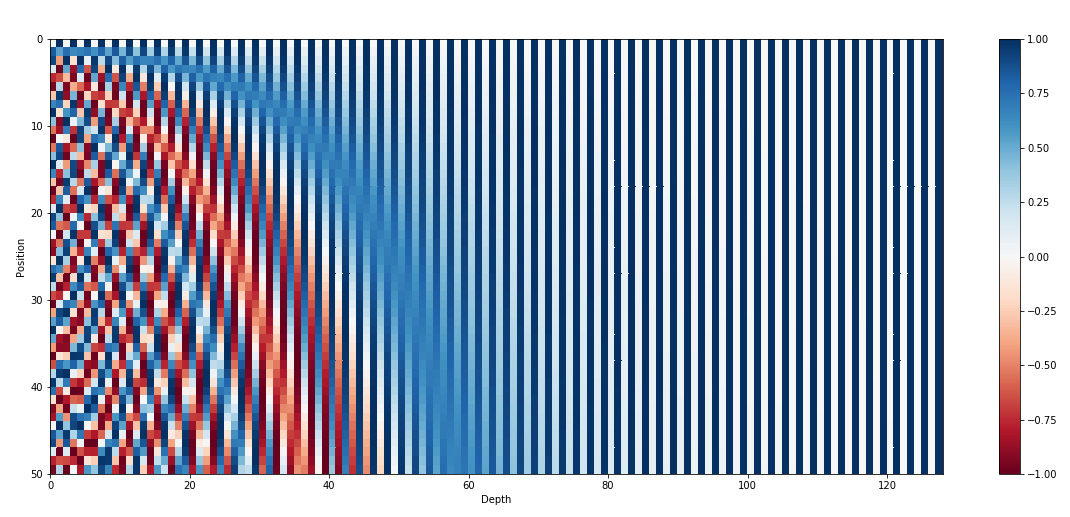
\includegraphics[width=.6\textwidth]{img/positional_encoding.png}
		\vspace{-.75em}
	\end{center} \pause
	Modern-day references: \textbf{\href{https://arxiv.org/abs/2104.09864}{Rotary Positional Encodings (RoPE)}}.
\end{frame}

\begin{frame}{Multi-Headed Setting}
	Each block of self-attention constitutes it's own head. \pause \newline \\

	Intuitively, \textbf{multiple interpretations are desired from a given input}. \\
	e.g: NER, Sentence-Structure Decomposition, POS tagging. \pause \newline \\

	Therefore, we instantiate \textit{multiple} heads within each layer, and concatenate to construct a final output represetnation.
	\begin{gather}
		MHA = \text{Concat}(\{h_i\}^H_{i=1})W_O
	\end{gather} \pause
	To keep computational costs consistent, we proportionally reduce the hidden dimension for each head:
	\begin{gather}
		W_{K, i}, W_{Q, i}, W_{V, i} \in \mathbb{R}^{d_{in} \times \nicefrac{d_{out}}{n_{head}}} \quad \forall i \in \{1, \ldots, n_{head}\}
	\end{gather} \pause
	Modern-day references: \textbf{\href{https://arxiv.org/abs/2205.14135}{Flash Attention}}, \textbf{\href{https://arxiv.org/abs/2502.07864}{Multi-Head Latent Attention}}.
\end{frame}

\begin{frame}{Self-Attention ($\nicefrac{2}{2}$)}
	\begin{center}
		\includegraphics<1>[width=\textwidth]{img/attention_1.pdf}
		\includegraphics<2>[width=\textwidth]{img/attention_2.pdf}
		\includegraphics<3>[width=\textwidth]{img/attention_3.pdf}
		\includegraphics<4>[width=\textwidth]{img/attention_4.pdf}
		\includegraphics<5>[width=\textwidth]{img/attention_5.pdf}
		\includegraphics<6>[width=\textwidth]{img/attention_6.pdf}
		\includegraphics<7>[width=\textwidth]{img/attention_7.pdf}
		\includegraphics<8>[width=\textwidth]{img/attention_8.pdf}
	\end{center}
\end{frame}

\begin{frame}{Feedforward MLP}
	Using attention, we now have an updated representation of our input. We now need to perform operations on this contextualized input to make inferences about our actual objective. \pause \newline \\

	For this, a two-layer MLP is instantiated that expands and consequently contracts the input dimension.
	\begin{gather}
		FFN(x) = \sigma_{relu}(xW_1 + b_1)W_2 + b_2
	\end{gather}
	The original paper uses a factor of $4$.
\end{frame}

\begin{frame}{Scaling to Deeper Networks -- A Better Interpretation}
	\begin{columns}
		\begin{column}{.35\textwidth}
			\begin{center}
				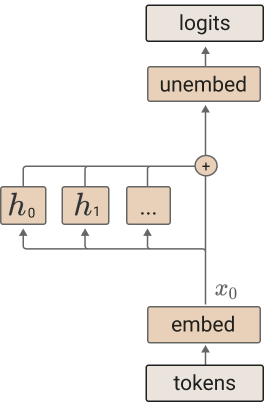
\includegraphics[width=\textwidth]{img/circuit-arch.png}
			\end{center}
		\end{column}
		\begin{column}{.5\textwidth}
			Deep neural architectures struggle with vanishing gradients, when trained at scale. \pause \newline \\

			The approach used universally is to add ``skip connections'' to maintain a short gradient path, and mitigate this concern. \pause \newline \\

			A result of this setup is that we can interpret each attention head and MLP as ``reading from'' and ``writing to'' a residual stream. \pause
		\end{column}
	\end{columns}
	\vspace{1em}
	In addition, we also perform layer normalization over the latent vectors before MLP \& self-attention.
\end{frame}

\begin{frame}{Inference \& Training}
	\textbf{Autoregressive Sampling:} The output of the model during a single forward pass is a token. added to the input, and the forward pass is run once again. This creates the final output, detokenized to a sentence. \pause \newline \\

	\textbf{Training:} Each token sequence $\{x_i\}^T_{t=1}$ contains $T-1$ targets.
	\begin{gather}
		\mathcal{L}_{CE}(\{x\}^T_{t=1}, \theta) = \frac{1}{T-1}\sum^{T-1}_{t' = 1} \mathcal{L}_{CE}(f_\theta(\{x_{t'+1} | x_t\}^{t'}_{t=1}), x_{t' + 1})
	\end{gather} \pause
	However, training these blocks means attention would be able to \textit{look into the future}. \pause We correct this by applying an upper-triangular causal mask:

	\begin{center}
		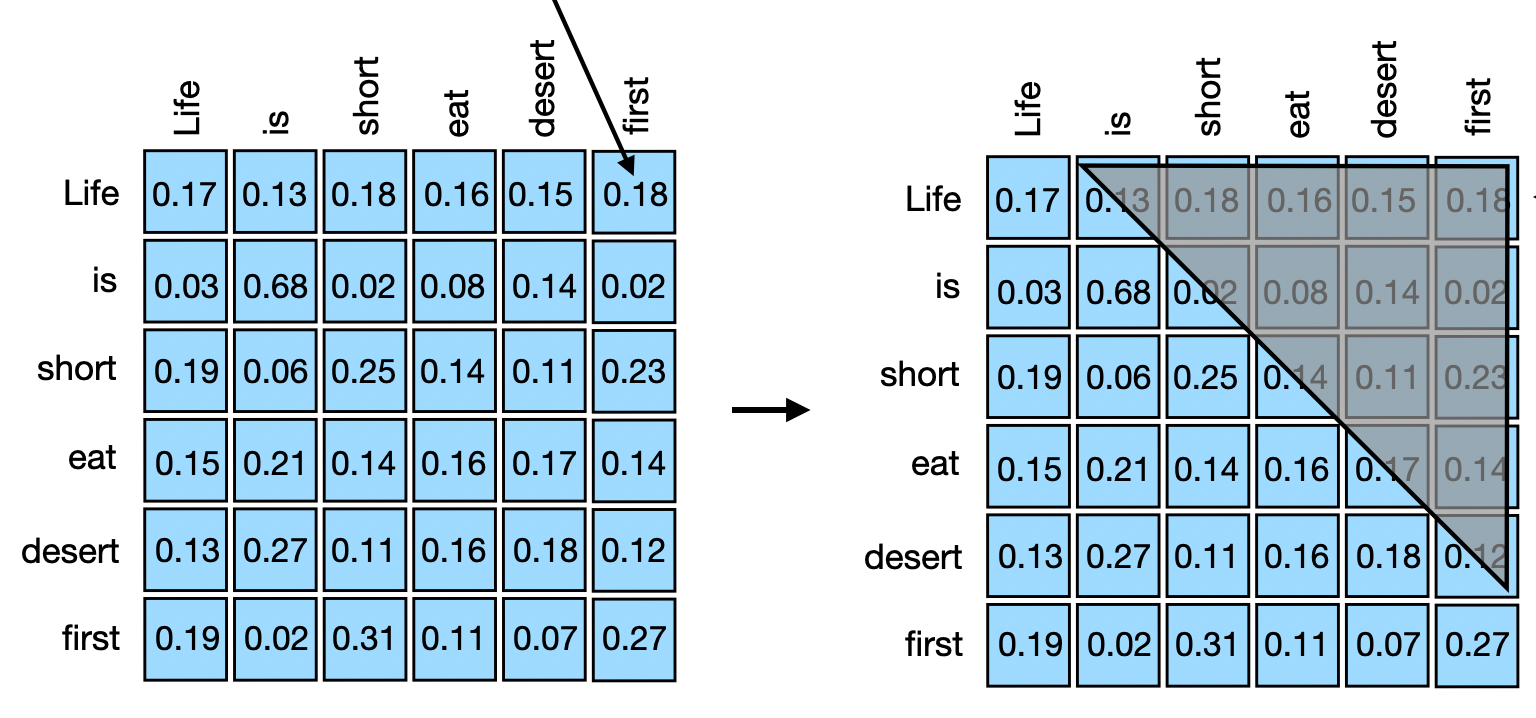
\includegraphics[width=.5\textwidth]{img/causal-mask.png}
	\end{center}
\end{frame}

\begin{frame}{Reviewing NanoGPT}
	\begin{center}
		If you can view this screen, I am making a mistake.
	\end{center}
\end{frame}

\begin{frame}{Thank you!}
	\begin{center}
		Have an awesome rest of your day!
	\end{center}
	\begin{center}
		\textbf{Slides:} {\small \url{https://cs.purdue.edu/homes/jsetpal/slides/transformer.pdf}}
	\end{center}
\end{frame}

\end{document}
